\section{Introdução}
\begin{frame}{Introdução}

%\centering
%\begin{minipage}{0.8\textwidth}

\begin{block}{Lógica Paraconsistente \tiny \cite{JoaoInacio}}
\begin{itemize}
\item Ferramenta promissora para tomada de decisão;
\item Robótica, Automação Industrial, IA, Logística, etc.
\end{itemize}
\end{block}

\begin{alertblock}{Ideia de uso da Lógica Paraconsistente \tiny \cite{JISF2011}}
\begin{itemize}
\item Conjunto de axiomas e regras de inferência;
\item Objetiva representar formalmente um raciocínio válido.
\end{itemize}
\end{alertblock}

%\end{minipage}
%\end{frame}


\end{frame}


%%%%%%%%%%%%%%%%%%%%%%%%%%%%%%%%%%%%%%% Objetivo
\begin{frame}{Objetivo(s)}
\begin{exampleblock}{Geral}
Estudar a LPA2v e desenvolver um algoritmo que possa ser embarcado para atuar no controle dinâmico de um sistema físico.
\end{exampleblock}

\begin{alertblock}{Específicos}
\begin{itemize}
\item Construir um sistema físico para o controle de velocidade em um motor CC.
\item Implementar o algorítmo da LPA2v e criar uma biblioteca.
\item Desenvolver a malha de controle do sistema físico proposto utilizando o algorítmo da LPA2v.
\end{itemize}
\end{alertblock}

\end{frame}



%%%%%%%%%%%%%%%%%%%%%%%%%%%%%%%%%%%%%%% Lógica Clássica
\begin{frame}{Lógica Clássica}
\begin{block}{A origem \tiny \cite{JoaoInacio}}
Grécia Antiga : \emph{Tópicos} de Aristóteles  340 a.C.
\end{block}
\begin{block}{Princípios da Lógica \tiny \cite{JoaoInacio}}

\begin{enumerate}
\item Princípio de Identidade: 
    \begin{math}
	A \rightarrow A 
	\textrm{ ou } 
	\forall x(x=x);
    \end{math}

\item Princípio do Terceiro Excluído:
    \begin{math}
	A \vee \neg A
	\textrm{ ou }
	\forall x(Ax \vee \neg Ax);
    \end{math}

\item Princípio da Não Contradição: 
    \begin{math}
	\neg (A \wedge \neg A)
	\textrm{ ou }
	\forall x\neg(Ax \wedge \neg Ax).
    \end{math}

\end{enumerate}


\end{block}
\end{frame}

%%%%%%%%%%%%%%%%%%%%%%%%%%%%%%%%%%%%%%% Lógica Paraconsistente
\begin{frame}{Lógica Paraconsistente}

\begin{block}{Criadores \tiny \cite{DecioKrause}}
\begin{itemize}
\item Newton Carneiro Affonso da Costa (1929-presente data)
\item Stanislaw Jaskiwski (1906-1965)
\end{itemize}
\end{block}

\begin{block}{Desenvolvimento: Costa, Subrahmanian e Vago \tiny \cite{DecioKrause}}
\begin{itemize}
\item Lógica Paraconsistente Anotada
\item extensão a uma Lógica de Predicados Paraconsistente Anotada de primeira ordem 
\end{itemize}
\end{block}

\end{frame}

%%%%%%%%%%%%%%%%%%%%%%%%%%%%%%%%%%%%%%% Lógica Paraconsistente Anotada
\begin{frame}{Lógica Paraconsistente Anotada de Anotação com dois valores (LPA2v) \tiny \cite{JoaoInacio}}

\begin{block}{
\centering 
$\tau = \{ ( \mu , \lambda ) \mid \mu ,\lambda \in [0,1] \subset \Re \}$
}
\end{block}
\vspace{0.4cm}
\begin{minipage}{0.40\linewidth}
\begin{figure}[!htb]
%\caption{Reticulado finito de Hasse}
\center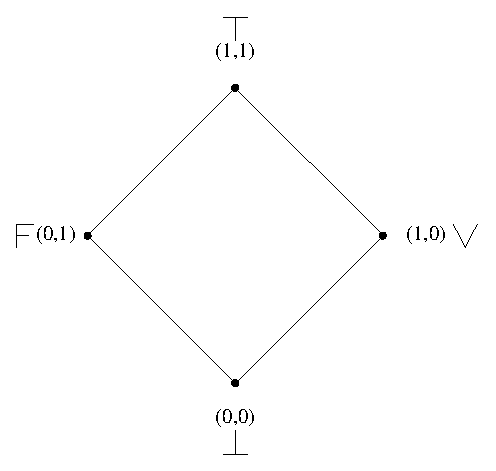
\includegraphics[scale=0.6]{./imagens/C421reticuladoHasse.eps}
\label{fig:reticuladoHasse}
%%%{\small Fonte: \cite{JoaoInacio} }
\end{figure}
\end{minipage}
\begin{minipage}{0.55\linewidth}
\center
\begin{itemize}
\item $(0,0) = \bot \Rightarrow $ Paracompleto;
\item $(0,1) = F \Rightarrow $ Falso;
\item $(1,1) = \top \Rightarrow $ Contradição;
\item $(1,0) = V \Rightarrow $ Verdade.
\end{itemize}
\end{minipage}

\end{frame}
%%%%%%%%%%%%%%%%%%%%%%%%%%%%%%%%%%%%%%% Proposição
\begin{frame}{A Proposição}
\vspace{1cm}

\begin{block}{}
\center
Para toda \textbf{proposição $P$} há um par de valores, \\
chamada de \textbf{anotação}, \textbf{$(\mu , \lambda )$}, onde \\
$\mu$ é o \textbf{grau de evidência favorável} e \\
$\lambda $ é o \textbf{grau de evidência desfavorável}, \\
representada como  \textbf{$P_{( \mu , \lambda )}$ }.
\end{block}

\end{frame}


%%%%%%%%%%%%%%%%%%%%%%%%%%%%%%%%%%%%%%% Quadrado Unitário no Plano Cartesiano
\begin{frame}{Quadrado Unitário no Plano Cartesiano}

\begin{block}{ \centering   $(\mu, \lambda ) \leftrightarrow (x,y) $ } \end{block}
\vspace{1cm}
\begin{minipage}{0.40\linewidth}
\begin{figure}[!htb]
%\caption{Representação do reticulado no quadrado unitário no plano cartesiano}
\center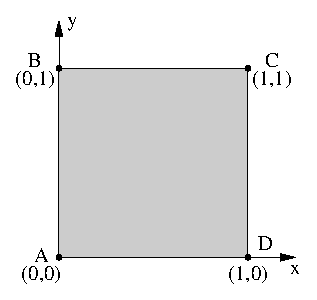
\includegraphics[scale=1.0]{./imagens/C422qupc.eps}
\label{fig:reticuladoQUPC}
%%%{\small Fonte: \cite{JoaoInacio} }
\end{figure}
\end{minipage}
\begin{minipage}{0.55\linewidth}
\center
\begin{itemize}
\item $A: (0,0) = \bot \Rightarrow $ Paracompleto;
\item $B: (0,1) = F \Rightarrow $ Falso;
\item $C: (1,1) = \top \Rightarrow $ Contradição;
\item $D: (1,0) = V \Rightarrow $ Verdade.
\end{itemize}
\end{minipage}

\end{frame}

%%%%%%%%%%%%%%%%%%%%%%%%%%%%%%%%%%%%%%% Reta Perfeitamente Definida
\begin{frame}{Reta Perfeitamente Definida}
\begin{block}{ \centering   $(\mu, \lambda ) \leftrightarrow (x,y) $ } \end{block}
\vspace{1cm}
\begin{minipage}{0.50\linewidth}
\begin{figure}[!htb]
%\caption{Representação da Reta Perfeitamente Definida}
\center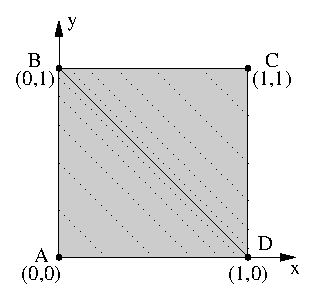
\includegraphics[scale=1.0]{./imagens/C424retaPerfeitamenteDefinida.eps}
%\label{fig:retaPerfeitamenteDefinida}
%%%{\small Fonte: \cite{JoaoInacio} }
\end{figure}
\end{minipage}
\begin{minipage}{0.45\linewidth}

\begin{itemize}
\item $\mu + \lambda = 1$
\item $\mu + \lambda - 1 = 0$
\item Grau de contradição
  \begin{itemize}
    \item $G _{ct} = \mu + \lambda - 1$
    \item $-1 \leqslant G _{ct} \leqslant 1$
  \end{itemize}
\end{itemize}
\end{minipage}

\end{frame}

%%%%%%%%%%%%%%%%%%%%%%%%%%%%%%%%%%%%%%% Reta Perfeitamente Indefinida
\begin{frame}{Reta Perfeitamente Indefinida}
\begin{block}{ \centering   $(\mu, \lambda ) \leftrightarrow (x,y) $ } \end{block}
\vspace{1cm}
\begin{minipage}{0.50\linewidth}
\begin{figure}[!htb]
%\caption{Representação da Reta Perfeitamente Indefinida}
\center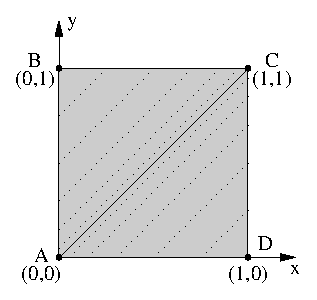
\includegraphics[scale=1.0]{./imagens/C426retaPerfeitamenteIndefinida.eps}
%\label{fig:retaPerfeitamenteDefinida}
%%%{\small Fonte: \cite{JoaoInacio} }
\end{figure}
\end{minipage}
\begin{minipage}{0.45\linewidth}

\begin{itemize}
\item $\mu - \lambda = 0$
\item Grau de certeza
  \begin{itemize}
    \item $G _{c} = \mu - \lambda$
    \item $-1 \leqslant G _{c} \leqslant 1$
  \end{itemize}
\end{itemize}
\end{minipage}

\end{frame}

%%%%%%%%%%%%%%%%%%%%%%%%%%%%%%%%%%%%%%% Representação do reticulado
\begin{frame}{\small{Representação do Reticulado da LPA2v subdividido em 12 regiões}}
\vspace{1cm}
\begin{minipage}{0.50\linewidth}
\begin{figure}[!htb]
%\caption{Representação dos valores de controle}
\center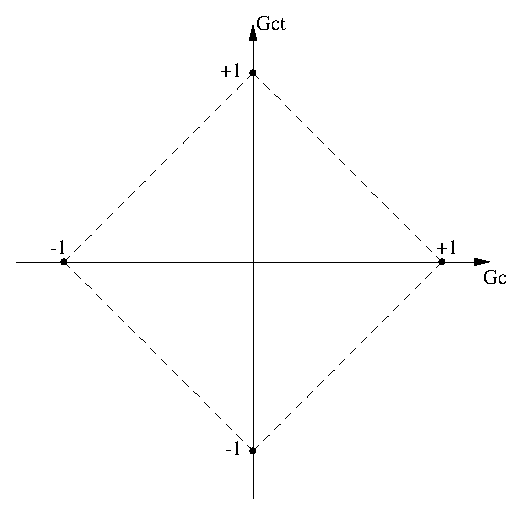
\includegraphics[scale=0.65]{./imagens/C428retasgcgct.eps}
\end{figure}
\end{minipage}
\begin{minipage}{0.45\linewidth}
\begin{figure}[!htb]
\center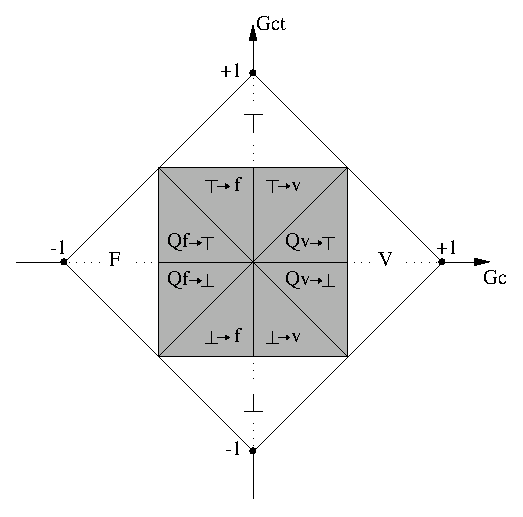
\includegraphics[scale=0.65]{./imagens/C430gcgct.eps}
%\caption{Representação do reticulado da LPA2v subdividido em 12 regiões}
\label{fig:reticuladoLPA2v}
\end{figure}
\end{minipage}

\end{frame}


